\section{Methodology}
% Method: Describe the model that you implement, the data set that you use, and any other
% materials. There should be sufficient details that another researcher is able to more or less
% replicate your experiment with some effort.

% The first line of the file must be
% \begin{quote}
% \begin{verbatim}
% \documentclass[11pt]{article}
% \end{verbatim}
% \end{quote}
% To load the style file in the review version:
% \begin{quote}
% \begin{verbatim}
% \usepackage[review]{ACL2023}
% \end{verbatim}
% \end{quote}



Our methodology is outlined in the following workflow, shown in \textit{Figure~\ref{fig:methods-overview}}.


\begin{figure}[h!]
    \centering
    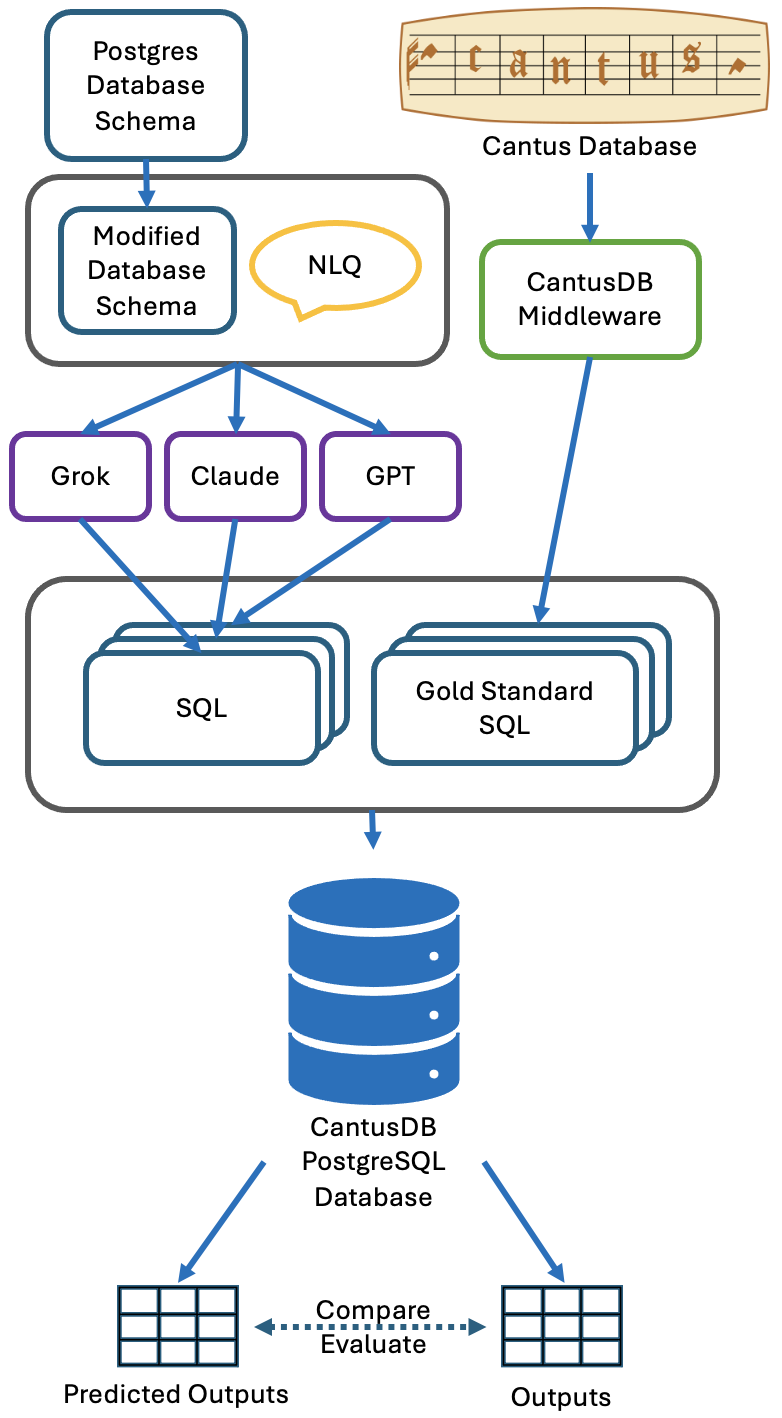
\includegraphics[width=0.45\textwidth]{workflow-vertical.png} % Adjust width as needed
    \caption{Overview of the methodology. Ground truth SQL queries are collected from Cantus Database. Natural language queries with a database schema are used to prompt various LLM's to generate SQL queries. The results are generated from a PostgreSQL database of CantusDB, and object ID values are compared and evaluated.}
    \label{fig:methods-overview} % Label for referencing the figure
\end{figure}

Firstly, ground truth data is collected from the Cantus Database site by using a local deployment of the website. Middleware is inserted into the codebase to extract SQL queries that are made on the database. These SQL queries are manually annotated with their corresponding natural language questions, which reflect the queries made on the site.

The context data provided to the large language model (LLM) consists of a modified version of the database schema and a natural language question. To generate the schema, we systematically process the PostgreSQL database dump using the following steps:

\begin{enumerate}
    \item Extract the database schema in a plain-text format using PostgreSQL's schema-only dump feature.
    \item Filter out only the table creation statements from the schema dump.
    \item Include essential constraints, such as primary keys, foreign keys, and references, to capture the relationships between tables.
    \item Remove duplicate entries to ensure a concise representation of the schema.
    \item Simplify the schema by removing non-essential modifiers, such as deferrable constraints.
    \item Clean up leading whitespace and other formatting inconsistencies to produce a compact, readable version of the schema.
    \item Integrate the fixed values into the database schema to produce the extended version.
\end{enumerate}

In the seventh step of the schema described above, we explore an extended version of the database schema. This extended schema introduces fixed values that are relevant for filtering data on the Cantus Database site but are not explicitly present in the raw schema dump. The purpose of including this extended schema is to evaluate whether incorporating such fixed values enhances the language model's ability to generate accurate SQL queries by providing richer context.

The fixed values include:
\begin{itemize}
    \item External identifiers for standard metadata repositories:
    \begin{itemize}
        \item RISM Online (1), VIAF (2), Wikidata (3), GND (4), Biblioth\`{e}que Nationale de France (5), Library of Congress (6), and DIAMM (7).
    \end{itemize}
    \item Source completeness statuses:
    \begin{itemize}
        \item Full Source, Fragment, Reconstruction, and Fragmented.
    \end{itemize}
    \item Additional prefixes used for inventory and source filtering:
    \begin{itemize}
        \item Temporary Prefixes: \texttt{``01--11, 16--17''}.
        \item Sanctuary Prefixes: \texttt{``12--15''}.
    \end{itemize}
    \item Proofreading status:
    \begin{itemize}
        \item Options include: Any, Yes, or No.
    \end{itemize}
\end{itemize}

By comparing the two schemas, we aim to determine whether the extended schema improves the language model's performance in understanding and generating accurate queries, particularly for tasks that rely on these fixed values for filtering and inventory purposes.

This refined schema serves as input context to the LLM, alongside a natural language question, allowing the model to focus on the relevant structural components of the database. The overall workflow ensures that the data preparation is efficient, systematic, and reproducible.



0. Dataset and other materials generated. Sincenot training or finetuning, don't need to have lots of data(LUCAS)
1. Why we need two separate schemas. Schema of the database and reducing into smal enough . Including the extra information - temporale sanctorale. (LUCAS)
2. Schema of the database without all the data crap (LUCAS)
2.5. Maybe discuss why the data and schema generation was manual.
3. Model: Have a diagram (google images) to showcase the workflow (LUCAS)
4. MOdel: Architecture .json, file structures (ZHANNA)
5. Discuss more in detail why these three models were chosen, more than the Introduction. (ZHANNA)
6. Evaluation metrics (CHARLES)
